\section{Gestion du jeu}

\subsection{Le monde des acteurs}

Pour manipuler le monde des acteurs, une structure \textbf{world} est créée qui regroupe l'ensemble des acteurs dans une liste.
\begin{lstlisting}[language={lisp},captionpos=b, frame=single]
(struct world (actors))
\end{lstlisting}
Cela permet de gérer de manière globale l'ajout des acteurs dans le jeu, les déplacements des acteurs, l'envoi des différents messages mais également la gestion des différentes collisions. \\
\begin{itemize}

    \item[\huge -]L'ajout d'une liste d'acteurs dans le monde se fait à l'aide d'une fonction
    \begin{lstlisting}[language={lisp},captionpos=b, frame=single]
    (world-add-actor world actors)
    \end{lstlisting}
    qui est de complexité en temps linéaire.
    
    \item[\huge -] En ce qui concerne les collisions rappelons qu'un acteur dispose d'une certaine durée de vie qui est constante et négative pour les acteurs ennemis du vaisseau allié mais positive et constante pour ce dernier. 
    Lors d'une collision du vaisseau principal et d'un autre acteur, un message de type \textbf{collide} qui est fonction du type du second acteur, est envoyé aux deux acteurs. Par la suite, à la mis à jour des acteurs le second est détruit et l'acteur principal gagne ou perd en durée de vie.
    Prenons l'exemple d'une collision avec un acteur \textbf{bonus}; dans notre cas nous considérons arbitrairement que ce dernier rapporte 3 unités de plus dans la durée de vie du vaisseau principal, contrairement à une collision avec un missile ennemi qui réduit de 2 unités sa duré de vie. \\
     Ainsi donc, afin de vérifier qu'il y' a des collisions dans le monde des acteurs, une fonction
    \begin{lstlisting}[language={lisp},captionpos=b, frame=single]
    (world-collision world)
    \end{lstlisting}    
    est implémentée. Elle prend récursivement un acteur du world et vérifie d'éventuelles collisions avec le reste des acteurs. S'il y' a collision, elle envoie le message \textbf{collide} aux deux acteurs et passe à un autre acteur, sinon refait la même démarche sur le reste des acteurs. Ce qui donne à cette fonction une complexité quadratique \textbf{$\theta (n^2)$} où n est le nombre d'acteurs dans l'espace de jeu.

    \item[\huge -] L'envoi des différents messages se fait à l'aide d'une fonction:
    \begin{lstlisting}[language={lisp},captionpos=b, frame=single]
    (world-send world msg type)
    \end{lstlisting}
    qui recherche de manière récursif dans world, les acteurs dont le type correspond à celui passé en paramètre et lui envoi le message msg à l'aide de la fonction \textbf{actor-send}. Cette fonction est de complexité en temps linéaire.
    
    \item[\huge -] La mis à jour du monde se fait à l'aide d'une fonction:
    \begin{lstlisting}[language={lisp},captionpos=b, frame=single]
    (world-update world)
    \end{lstlisting}
    qui utilise la fonction \textbf{actor-update} récursivement sur le world mais aussi la fonction \textbf{world-collision} ce qui lui donne d'ailleurs une complexité en temps quadratique.
\end{itemize}
Notons par ailleurs qu'il arrive un moment où certains acteurs sortent du cadre du jeu. Arrivés à l'abscisse 0, ces derniers doivent être détruits vue qu'ils sont arrivés à l'autre extrémité du cadre et qu'ils ne sont plus utiles dans la suite du jeu. La fonction \textbf{(destroy-actor actors)} le fait récursivement sur les différents acteurs. Elle vérifie également que le vaisseau principal se trouve à tout moment dans l'espace du jeu. S'il arrive qu'il sorte du cadre, ce dernier est détruit et le jeu prend fin.


\subsection{Avancement du jeu}
La structure world citée précédemment est placée dans une autre nommée \textbf{runtime} qui contient des messages et l'horloge globale \textbf{tick}. Elle a pour fonction d'envoyer les différents messages aux acteurs du monde \textbf{world} à chaque pas de l'horloge, de les mettre à jour et de renvoyer un nouvel état du monde.

\begin{lstlisting}[language={lisp},captionpos=b, frame=single]
(struct runtime (world messages tick))
\end{lstlisting}

Au début du jeu, le seul acteur présent est le vaisseau principal attendant l'invasion des différents vaisseaux ennemis. A chaque pas de l'horloge \textbf{tick} et avant le prochain pas:
\begin{itemize}
    \item Le runtime ajoute dans son \textbf{world} des nouveaux acteurs, fournis par \textbf{(generate-actor tick)}, à l'aide de la fonction 
    \begin{lstlisting}[language={lisp},captionpos=b, frame=single]
    (runtime-add-actor runtime actors)
    \end{lstlisting}.
    
    \item le runtime par la suite reçoit une liste de messages  par la fonction 
    \begin{lstlisting}[language={lisp},captionpos=b, frame=single]
    (runtime-receive runtime messages)
    \end{lstlisting} avec \textbf{messages} de la forme \textbf{(list (msg type))} où chaque message \textbf{msg} est de type \textbf{move} à envoyer à l'acteur de type \textbf{type}. Cela à pour but de faire avancer d'un pas les différents acteurs.
    
    \item Après avoir reçu ses messages, le runtime vide son champs messages et envoie ces derniers aux différents acteurs à l'aide de la fonction 
    \begin{lstlisting}[language={lisp},captionpos=b, frame=single]
    (runtime-send runtime)
    \end{lstlisting}
    
    \item Enfin le runtime, à l'aide de la fonction
    \begin{lstlisting}[language={lisp},captionpos=b, frame=single]
    (runtime-update runtime)
    \end{lstlisting}, met à jour tout les acteurs et renvoie un nouvel état du monde.
\end{itemize}
Ces étapes sont effectuées successivement à chaque pas de l'horloge globale du jeu.
Toutes les fonctions citées plus haut sont linéaires à l'exception de la fonction de mise à jour qui est quadratique et de la fonction runtime-receive qui est constante.


\subsection{L'interface graphique}


L'affichage des acteurs ainsi que l'interface graphique est faite à l'aide de la bibliothèque \textbf{raart} qui fournie plusieurs fonctions permettant d'afficher du texte sur un terminal.
Pour l'animation du jeu c'est la bibliothéque \textbf{Lux} qui est utilisée. Elle fournit un moyen efficace de créer des programmes interactifs en temps réel. Pour le fonctionnement de la bibliothéque sur notre projet, il s'agit de créer une structure qui représente l'état globale de l'application.
\begin{lstlisting}[language={lisp},captionpos=b, frame=single]
    (struct game (runtime)
    #:methods lux:gen:word)   
\end{lstlisting}
La structure \textbf{game} comprend le runtime ainsi que différentes méthodes qui permettent la gestion de l'état du jeu:
\\

\begin{itemize}
    \item[\huge *] la méthode (word-fps w) renvoie le taux de mise à jour souhaité pour le \textbf{game} en images par seconde.
    
    \item[\huge *] la méthode (word-label w) renvoie le titre de la fenêtre contenant le jeu.
    
    \item[\huge *] la méthode (word-event w e) qui à partir d'un état du monde et d'un évènement \textbf{e} renvoie un nouvel état du monde. C'est cette méthode qui permet l'interaction entre le jeu et l'utilisateur.C'est ainsi que pour faire déplacer le vaisseau principal, l'utilisateur tape sur les touches de direction de son clavier et cette fonction envoie un message move ou shoot à l'acteur principal en fonction de la touche enfoncé sur le clavier. Rappelons par contre que seul le vaisseau principal est manipulable par l'utilisateur; le reste des acteurs est gérer par le runtime.
    
    \item[\huge *] la méthode (word-output w) qui permet d'afficher n'importe quel objet graphique.
    
    \item[\huge *] la méthode (word-tick w) qui permet la mise à jour des différents acteurs et renvoie un nouveau monde.
    
    \item[\huge *] la méthode (word-return w) qui affiche un message en cas d'éventuelles erreurs.
  \\  
\end{itemize}

\begin{figure}[h]
    \centering
    \label{fig:actor}
    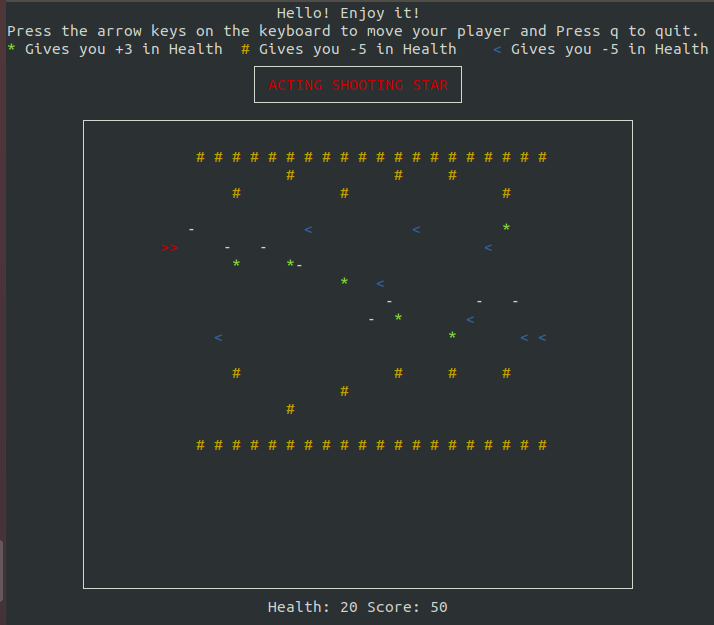
\includegraphics[width=0.9\textwidth]{Images/actor.png}
    \caption{L'interface graphique du jeu}
\end{figure}

A partir de la figure 1 nous pouvons visualiser la manière dont sont représentés nos différents acteurs:
\\

\begin{itemize}
    \item \textcolor{red}{\huge >>} représente l'acteur principal,
    \item \textcolor{blue}{\large <} représente un vaisseau ennemi et fait perdre 2 unités de vie au vaisseau principal,
    \item \textcolor{gray}{\huge -} représente un missile et fait perdre également 2 unités de vie au vaisseau principal,
    \item \textcolor{orange}{\#} représente un acteur obstacle. Il fait perdre 5 unité de vie au vaisseau principal,
    \item \textcolor{green}{\large *} représente un bonus et fait gagner 3 unités de vie au vaisseau principal
\end{itemize}



